\chapter{Realisierung}
% Dies ist das Hauptkapitel Ihrer Arbeit! Hier wird die Umsetzung der eigenen Ideen und Konzepte
% (Kapitel 3) anhand der gewählten Methoden (Kapitel 4) beschrieben, inkl. der dabei aufgetretenen
% Schwierigkeiten und Einschränkungen.

Wie im Kapitel \ref{vorgehen} Vorgehensmodell beschrieben, wurde die Arbeit während mehreren Sprints realisiert.
In den folgenden Abschnitten wird das Vorgehen während er einzelnen Sprints aufgezeigt.
Dabei werden die bearbeiteten User Stories beschrieben, Entscheidungen und Designs dokumentiert sowie aufgetretene Schwierigkeiten gezeigt.
Die sechs Sprints sowie die Vorbereitungsphase fanden während folgenden Zeiten statt:

\begin{itemize}
   \item Vorbereitungsphase 14.02. - 27.02.
   \item Sprint 1 18.02. - 13.03.
   \item Sprint 2 14.03. - 27.03.
   \item Sprint 3 28.03. - 10.04.
   \item Sprint 4 11.04. - 24.04.
   \item Sprint 5 25.04. - 08.05.
   \item Sprint 6 09.05. - 22.05.
\end{itemize}

\section{Vorbereitungsphase}
Die Arbeiten am Projekt begannen mit der Vorbereitungsphase. Das Zeil dieser war es, wichtige Abklärungen zu machen und Entscheidungen zu treffen damit im ersten Sprint mir der eigentlichen Entwicklung begonnen werden konnte.
Dies beinhaltete zum einen eine Befragung potenzieller Benutzer der zu entwickelnden Applikation sowie die Evaluation eines geeigneten Technologiestacks.
Mit einer Dauer von zwei Wochen war die Vorbereitungsphase gleich lang, wie ein Sprint. Bei ihr handelt es sich jedoch nicht um einen richtigen Sprint, da noch kein Backlog mit User Stories vorhanden war.
Der Backlog für die Sprints wurde währen dieser Phase basierend auf den Erkenntnissen der zuvor genannten Punkte erstellt.
In den folgenden Abschnitten wird die Umsetzung der Vorbereitungsphase detailliert beschrieben.

\subsection{DlmsQuickAccess}
Für die Erstellung des Projekts in \ac{ADO}, für das Git-Repository sowie für die C\# Solution wurden jeweils Namen benötigt.
Dazu wurde \textit{DlmsQuickAccess} kreiert.
Der Name ist an die zu ersetzende Funktion des \ac{DMT2}, \textit{Quick Access}, angelehnt.

\subsection{Kennenlernen der Nutzer}\label{survey}
Wie im Kapitel \ref{erwarteteResultate} erklärt, ist das Ziel dieses Projekts, die bestehende Anwendung, \textit{DMT2}, durch einen Neuentwicklung zu ersetzen.

Am Standort Cham der Landis+Gyr gibt es zwei Entwicklerteams, welche den \ac{DMT2} regelmässig verwenden.
Für dieses Projekt wurden die Mitglieder dieser beiden Teams als Nutzer definiert und in dieser Arbeit so bezeichnet.  % chamer das besser formuliere?
Um die Nutzer besser kennen zu lernen, wurden die Methoden \textit{Fokusgruppe} (\ref{fokusgruppe}) und \textit{Befragung} (\ref{befragung}) eingesetzt.

Zu Beginn der Vorbereitungsphase wurden alle Nutzer zu einer Gruppendiskussion eingeladen, um eine Fokusgruppe zu bilden.
In dieser Diskussion wurden erörtert, welche Dinge bei der bestehende Anwendung bereits gut funktionieren und welche als störend wahrgenommen werden.
Ebenfalls wurde von den Nutzern Ideen \& Wünsche für die Neuentwicklung abgeholt.

Für das sammeln der Antworten wurde während der Diskussion retrotool.io \footnote{https://retrotool.io/8mWyxCzpbIfQPydp2FPf4} eingesetzt.
Die Abbildungen \ref{fig:WhatWorksWell}, \ref{fig:WhatBothersYou} und \ref{fig:IdeasAndWishes} sind Screenshots daraus.

% todo In einem anderen Kapitel die Resultate der Umfrage aufarbeiten und hier referenzieren
% https://retrotool.io/8mWyxCzpbIfQPydp2FPf4


\begin{figure}[H]
   \centering
   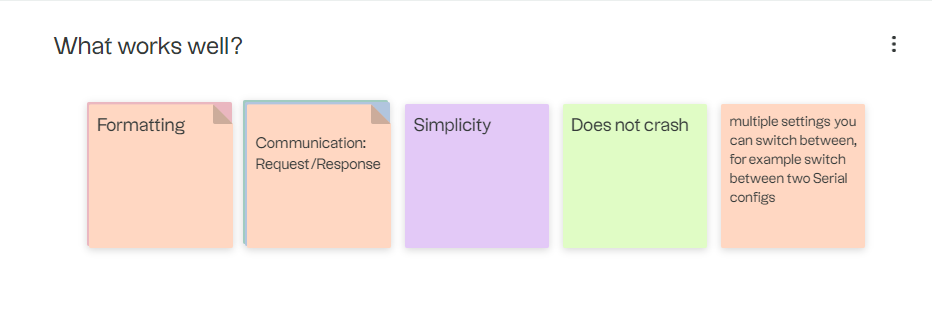
\includegraphics[width=1.0\textwidth]{gfx/S1_RetroBoard_WhatWorksWell.png}
   \caption{
       Antworten der Nutzer zur Frage "Was funktioniert bereits gut?"
   }
   \label{fig:WhatWorksWell}
\end{figure}

\begin{figure}[H]
   \centering
   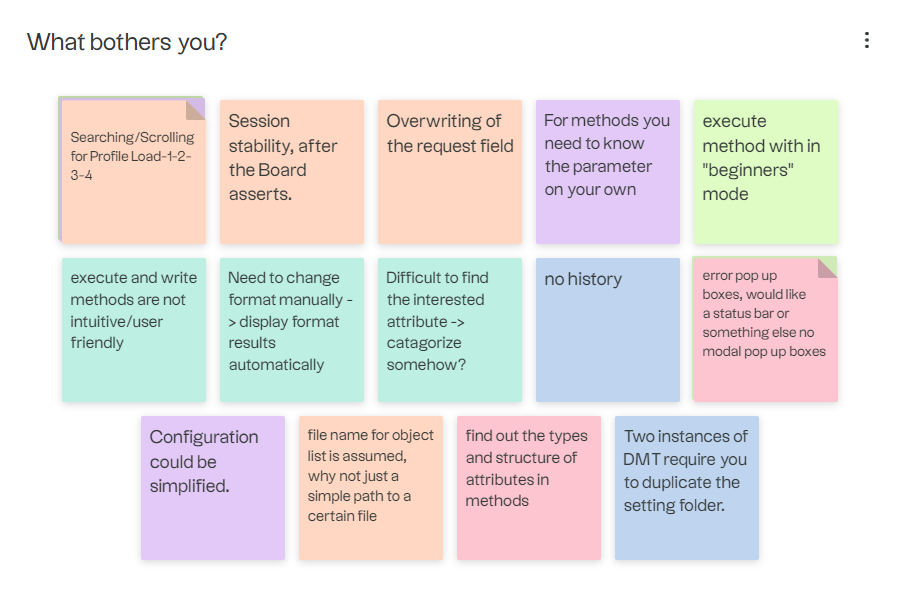
\includegraphics[width=1.0\textwidth]{gfx/S1_RetroBoard_WhatBothersYou.png}
   \caption{
       Antworten der Nutzer zur Frage "Was stört dich?"
   }
   \label{fig:WhatBothersYou}
\end{figure}

\begin{figure}[H]
   \centering
   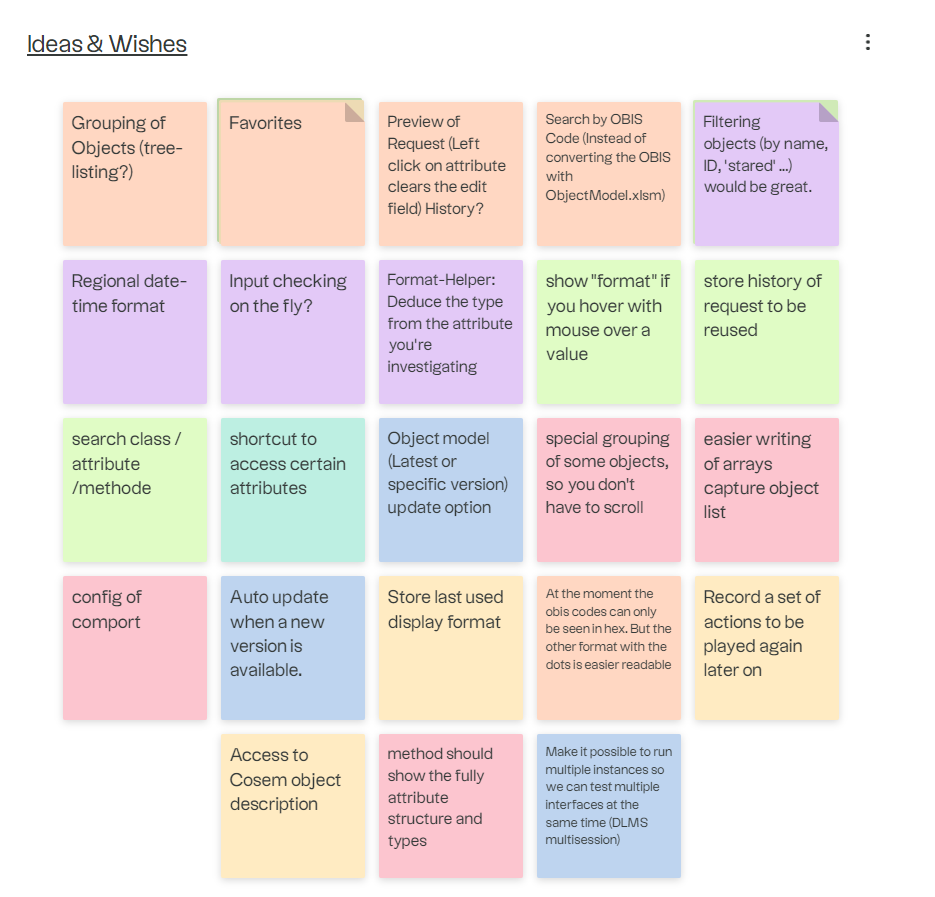
\includegraphics[width=1.0\textwidth]{gfx/S1_RetroBoard_IdeasAndWishes.png}
   \caption{
       Ideen und Wünsche der Nutzer an die neue Anwendung.
   }
   \label{fig:IdeasAndWishes}
\end{figure}
Anschliessend an dies Diskussion in der Fokusgruppe wurde eine Befragung mithilfe einer Online-Umfrage durchgeführt.
Das Ziel dieser ware es, quantitative Daten zu erheben.
Die Resultate der Umfrage sind dieser Arbeit im Anhang \ref{anhang:survey} beigelegt.
So mussten die Nutzer zehn mögliche Features, welche auf den von ihnen eingebrachten Ideen \& Wünsche basieren, priorisieren.


\begin{figure}[H]
   \centering
   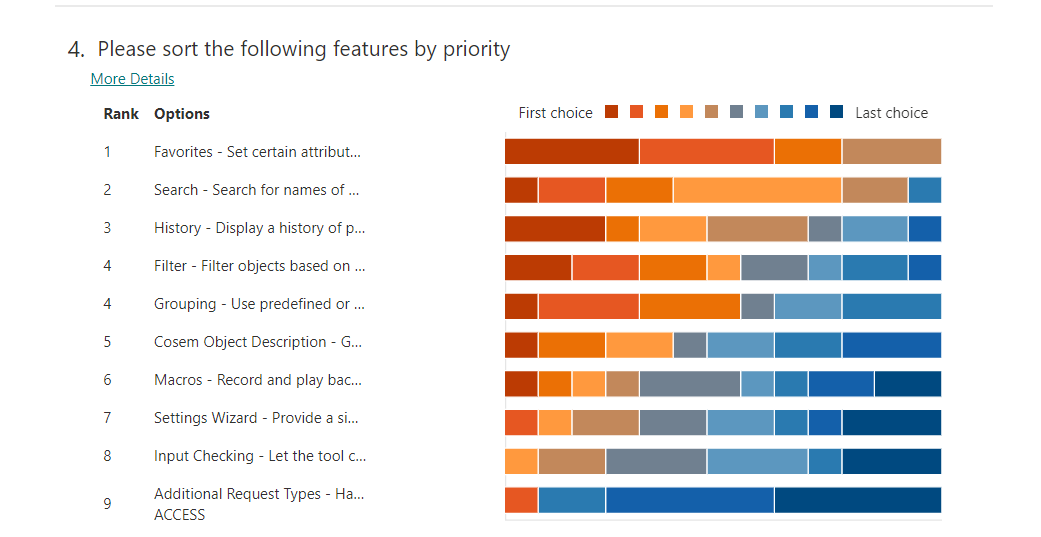
\includegraphics[width=1.0\textwidth]{gfx/S1_Survey_Prio.png}
   \caption{
       Resultat der Umfrage: Sortiere diese Features nach Priorität
   }
   \label{fig:FeaturesPrio}
\end{figure}

Die Nutzer wurden ebenfalls dazu befragt, auf welchen Plattformen sie die neue Anwendung gerne einsetzten würden.
Im nächsten Abschnitt werden die Antworten (Abbildung \ref{fig:SurveryPlatforms}) auf diese Frage sowie viele weitere Aspekte für die Evaluation des Technologiestacks verwendet.

\begin{figure}[H]
   \centering
   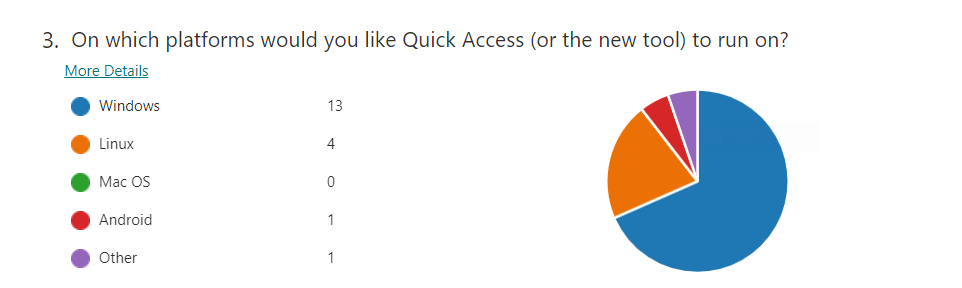
\includegraphics[width=1.0\textwidth]{gfx/S0_Survey_Platform.png}
   \caption{
       Resultat der Umfrage: Gewünschte Plattformen
   }
   \label{fig:SurveryPlatforms}
\end{figure}

\subsection{Evaluation des Technologiestacks}
Um im ersten Sprint mit der Implementation der Applikation beginnen zu können, musste zuerst ein geeigneter Technologiestack evaluiert werden.
Die im vorherigen Abschnitt erwähnt Umfrage hat ergeben, dass sich alle Befragten Windows als Zielplatform der neuen Anwendung wünschen.
Nur vereinzelt wurde nebst Windows noch Android oder Linux angegeben.

Im Projektauftrag (Anhang \ref{anhang:aufgabenstellung}) ist festgehalten, dass die Technologien frei gewählt werden können, für die Landis+Gyr jedoch günstig zu unterhalten sein soll.

Um dies zu erreichen, wurden für die Evaluation nur Programmiersprachen in Betracht gezogen, welche bei der Landis+Gyr bereits aktiv verwendet werden.
Im Kapitel \ref{lgintern} werden einige Anwendungen und Softwareprojekte der Landis+Gyr, welche im Umfeld der zu entwickelnden Anwendung betrieben und unterhalten werden, genauer beschrieben.
Die dort verwendeten Programmiersprachen sind C\#, Python und C++.


Ein wichtiger Teil der Anwendung wird die \ac{DLMS} Kommunikation mit den Stromzählern sein.
Diese ist in allen drei zuvor genannten Programmiersprachen bereits implementieren und wird in den Tools \textit{ATS}, \textit{libpydlms} rsp. \textit{DMT2} verwendet.
Da der \textit{DMT2} jedoch von einem externen Lieferanten entwickelt wurde, erlaubt die zugehörige Lizenz die Verwendung des Codes nicht ohne weiteres.


Der Fokus der zu entwickelnden Anwendung liegt auf der Benutzerschnittstelle.
Python Applikationen mit Benutzerschnittstelle gibt es bei der Landis+Gyr keine.
Möglich wäre ein Technologiestack bestehend aus Python Backend mit einem Angular \footnote{https://angular.io} Frontend.
Das Web-Framework Angular, welches mit der Sprache TypeScript verwendet wird, wird im Projekt \textit{Test Script Manager} eingesetzt.
Dieses Projekt wird an einem Standort ausserhalb der Schweiz entwickelt.
Als Backend wird dort jedoch nicht Python sondern C\# eingesetzt.
Eine Python+Angular Stack wäre somit neu für die Landis+Gyr, die einzelnen Technologien jedoch bereits etabliert.

Im Gegensatz zu Python existieren bei der Landis+Gyr bereits mehrere C\# Anwendungen, welche über eine Benutzerschnittstelle verfügen.
\textit{PicParted} und \textit{DocTool} sind C\# Anwendungen welche eine \ac{WPF}\footnote{https://docs.microsoft.com/en-us/visualstudio/designers/getting-started-with-wpf?view=vs-2022} Benutzerschnittstelle haben.
Sie werde im Bereich des Picasso Projekts \ref{picasso} eingesetzt und Unterhalten. 
Ursprünglich wurden sie vom Autor dieser Arbeit entwickelt.

Die Anwendung \textit{ATS}, welche im Abschnitt \ref{ats} genauer beschrieben wird, verfügt über Code für die \ac{DLMS} Kommunikation mit Stromzählern.
Dieser könnte für die neue Anwendung wiederverwendet werden.
Die in Abschnitt \ref{objectModelsClassDescriptions} beschriebenen Tools verfügen ebenfalls über C\# Code, welcher thematisch nahe an der neuen Anwendung ist und evtl. ebenfalls wiederverwendet werden kann.

Aufgrund der genannten Umstände viel die Entscheidung auf einen C\# Technologiestack.
Ein weitere Vorteil von C\# ist, dass die Sprache, wie in Abschnitt \ref{typing} erwähnt, über eine statische sowie dynamische Typenüberprüfung verfügt.
% TODO WinUI3 Evaluation beschreiben

Um im ersten Sprint direkt mit der Entwicklung loslegen zu können wurde in \ac{ADO} ein Repository erstellt.
Dieses wurde mit einer leeren WinUI3 Projekt initialisiert.




\subsection{Erstellung des Backlogs}
Wie in Abschnitt \ref{methoden:ADO} erklärt, wurde \ac{ADO} für die Verwaltung des Backlogs verwendet.
Dazu musste als erstes eine neues \ac{ADO} Projekt erstellt und die Sprints eingetragen werden.
Nun konnten User Stories formuliert und auf die sechs geplanten Sprints verteilt werden.
Welche Stories im ersten Sprint bearbeitet wurden und wie dies genau ablief ist im folgenden Kapitel zu lesen.
% TODO no chli meh schribe?
\newpage

\section{Sprint 1}
Im ersten Sprint wurde der Grundstein für das Projekt sowie die Applikation gelegt.


\section{Schwierigkeiten}
Benutzen von Shims mittels Microsoft Fakes
% https://docs.microsoft.com/en-us/previous-versions/visualstudio/visual-studio-2015/test/isolating-code-under-test-with-microsoft-fakes?view=vs-2015&redirectedfrom=MSDN

\subsection{Build}
<RuntimeIdentifiers>win10-x86;win10-x64;win10-arm64</RuntimeIdentifiers> vs <RuntimeIdentifiers>win-x64</RuntimeIdentifiers>
Probleme beim Build via msbuild Kommando und im CI/CD

Probleme beim ausführen von tests via vstest.console.exe
"Could not find testhost"
Dieses Problem tritt ebenfalls auf, wenn ein neues Testprojekt erstllt wird und dies mit vstest abgespielt wird.

Lösung:
dotnet cli verwenden. neuses Problem:  The imported project "C:\\Program Files\\dotnet\\sdk\\6.0.200\\Microsoft\\DesktopBridge\\Microsoft.DesktopBridge.props" was not found.
Lösung:
neue Solution nur mit Test projekten

\section{CI/CD}

\subsection{Schwierigkeiten}
Die Azure DevOps Instanz der Landis+Gyr wird global verwaltet. Für neue Projekte, Anpassungen und Berechtigugen mussten jeweils die entsprechenden Prozesse eingehalten werden. (SP/Azure work item)
Projekt
Pipeline erstellen
Agent
Agent mit VS 2022

Workaround VS 2022 nicht gefunden
https://stackoverflow.com/questions/70174595/visual-studio-2022-not-listed-in-devops-build-solution-pipeline-task

Secure File für Zertifikat
-> Vorerst wurde der Private Key in das Repository eingecheckt, da keine Secure Files erstellt werden können. Verantwortlicher ist in den Ferien.


\subsection{InfraLib}
Parsen von ClassDescriptions kaum getestet. Xml node hat im Code einen anderen Namen als in den Dateien.

Neue tests für InfraLib schreiben und code fixen.

\subsection{Adapter Pattern}

Mithilfe des Adapter Pattern wurde die bestehende Klassenstrukture der InfraLib auf die benötigten Interfaces adaptiert.
Dies erlaubte es, die Interfaces genau so zu modellieren, wie sie für den DlmsQuickAccess benötigt werden.
Dependency auf InfraLib ist an einem Ort.


\section{Entscheidungen}

Mock Framework:
https://github.com/moq/moq4


Logging Framework
log4Net, weil es bereits für InfraLib verwendet wird. 

https://stackoverflow.com/questions/53092470/how-to-configure-logging-via-log4net-in-an-uwp-app

\section{Globaler Exception Handler}

Exceptions, welche vom Programm nicht abgefangen werden und zu einem Absturz der Anwendung führen, werden von einem globalen Exception Handler gefangen.
Dieser schreibt deren auftreten in die Log-Datei. Für vereinfachtes Troubeshooting, wir diese Log Datei auch sofort geöffnet. Das Programm stürtzt danach ab.

Limitierugen:
Exception, welche im Aufbau der Anwendung vorkommen. Also beispielsweise im XAML oder im Konstruktor eines ViewModels können nicht abgefangen werden.
https://docs.microsoft.com/en-us/windows/winui/api/microsoft.ui.xaml.application.unhandledexception?view=winui-3.0


\section{Versionen von .net}
WinUI3 benötigt spezifische Version net6.0-windows10.0.19041.0.
Test Projekt muss ebenfals diese als TargetFramwork haben.
Wenn dieses ausgewählt wird könne jedoch keine UT mehr ausgeführt werden.

UWP UnitTest Projekt hilft auch nicht

Lösung:
Eigenes Projekt für VM und so




UnitTest:

Internal Classes testen:
https://stackoverflow.com/questions/358196/c-sharp-internal-access-modifier-when-doing-unit-testing

\section{Dummy Klassen}
Für das Testig von Picasso Tool wurde Dummy CosemKlassen erstellt, welche diverse Edge-Cases abdekend.
Diese sind sehr praktisch für das entwickeln und testen der Anwendung.


\section{Sprint resultat}
Nur 2 stories fertig.


nichts fertig
Release funktioniert noch nicht
Unittest laufen noch nicht

Damit erster release n


\newpage
\section{Sprint 2}
Im zweiten Sprint wurden Arbeiten, welche im ersten Sprint begonnen wurden, abgeschlossen.
Die zuvor erstellten Funktionen wurden zusammengeführt und erweitert.
Konkret wurde diesen Stories gearbeitet:
\begin{itemize}
   \item Die Applikation soll auf \ac{ADO} bei jedem neuem Commit automatisch gebaut und getestet werden. 
   \item Werte von Attributen sollen vom Zähler ausgelesen und in der Benutzerschnittstelle dargestellt werden.
   \item Die Benutzerschnittstelle soll das Schrieben von Attributwerten sowie ausführen von Methoden unterstützen.
\end{itemize}


\subsection{Build bei Commit}\label{s2:buildOnCommit}
Die Arbeiten an dieser Story wurden bereits im vorherigen Sprint begonnen.
Das Ziel der Story und das bisherige Vorgehen ist im Abschnitt \ref{story_buildoncommit} aufgeführt.
Die Pipeline in \ac{ADO} wurde nun so konfiguriert, dass die Solution kompiliert wird.
Dies funktionierte problemlos.
Als die Pipeline um einen Task erweitert wurde, welcher die Tests ausführen soll traten Schwierigkeiten auf.
Im Log war der Fehler \dq  Could not find testhost\dq , ausgelöst von \textit{vstest.console.exe}, zu lesen.
Da die Unittests lokal jeweils über Visual Studio ausgeführt wurde, trat dieser Fehler lokal nicht auf.
Er konnte jedoch reproduziert werden, indem \textit{vstest.console.exe} analog zur Pipeline aufgerufen wurde.
Ein Test mit einem neuen, leeren Projekt zeigte, dass es sich dabei um einen Fehler von Visual Studio handelt.

Dieses Problem konnte umgangen werden, indem anstelle von msbuild\footnote{https://docs.microsoft.com/en-us/visualstudio/msbuild/msbuild?view=vs-2022}
die .NET CLI\footnote{https://docs.microsoft.com/en-us/dotnet/core/tools/} verwendet wurde.
Bei der Verwendung der .NET CLI trat ein neues Problem auf.
Diese Unterstützt das Kompilieren von WinUI3 Anwendungen nicht.
Da, wie bereits in Abschnitt \ref{objectModelDevSchwierigkeiten} erklärt, bei den Unittest gar keine Abhängigkeiten zu WinUi3 bestehen können ist dies nicht weiter tragisch.
Damit das Kompilieren erfolgreich funktioniert, wurde eine zweite Solution erstellt, welche nur jene C\# Projekte enthält, die nicht von WinUI3 abhängen.

So konnte die Story trotz diverser Schwierigkeiten fertiggestellt werden.

\subsection{Lesen von Attributen}
\dq Werte von Attributen sollen vom Zähler ausgelesen und in der Benutzerschnittstelle dargestellt werden.\dq
\subsubsection{Ziel}
Im ersten Sprint wurde die Kommunikation mit den Stromzählern implementiert.
Ebenfalls wurde eine Visualisierung des Object Models zur Benutzerschnittstelle hinzugefügt.
Diese Dinge sollen nun so kombiniert werden, dass im Object Model ein Attribute angewählt werde kann und diese über einen Klick ausgelesen wird.
Die Werte sollen dabei jeweils direkt im Object Model angezeigt werden.
Die Story gilt als erledigt, wenn Attribute inklusive Arrays und Strukturen korrekt ausgelesen und dargestellt werden können.

\subsubsection{Vorgehen und Schwierigkeiten}
Für das Auslesen von Attributen kann das \textit{IRawReader} Interface verwendet werden.
Dieses wird von der in Sprint 1 implementierten Klasse \textit{ReaderWriter} implementiert.
Der Methode Read() wird ein Short Name als Parameter mitgegeben und sie gibt den ausgelesenen Wert als string zurück.
Beim Short Name handelt es sich um eine Kombination aus Objektname und Attributname welche ein bestimmtes Attribut eindeutig identifizieren.
Die Werte werden in einem proprietären Format zurückgegeben. 
Dieses sieht beispielsweise wie folgt aus:
\begin{verbatim}
   Struct[3](
      Integer16('0005')
      OctetString[6]('112233445566')
      Integer8('01')
   )'
\end{verbatim}
\begin{figure}
\centering
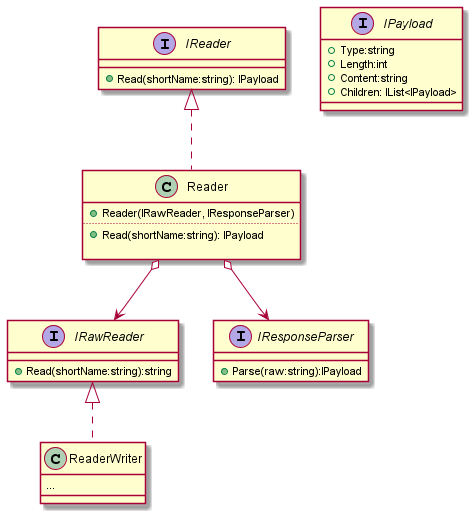
\includegraphics[width=0.7\textwidth]{gfx/string_toPayload.png}
\caption{
   Klassendiagramm zur Reader Klasse
   }
   \label{fig:reader}
\end{figure}
Diese Struktur wurde durch das Interface \textit{IPayload} repräsentiert.
Die Klasse \textit{Reader}, welche im Klassendiagramm \ref{fig:reader} dargestellt ist, liest Werte aus dem Zähler aus und gibt diese als \textit{IPayload} zurück.
So kann in der Applikationslogik vereinfacht gelesen und auf die Antwort zugegriffen werden.

Die Datentypen der Attribute lassen sich in die Kategorien einfach und komplex einteilen.
Zu den einfachen Typen gehören strings und numerische Typen wie Integer oder Float.
Arrays und Strukturen sind komplexe Typen.
Um einen einfachen Typen in der Benutzeroberfläche darzustellen, reicht eine Textbox aus.
Eine Struktur setzt sich jedoch jeweils aus mehreren Werten zusammen und benötigt deshalb für die Darstellung auch mehrere Textboxen.
Die genaue Angaben zu den Typen sind im Objekt Model nicht vorhanden.
Der Antwort, welche beim Lesen eines Attributs zurückgegeben wird beinhaltet Angaben zum Aufbau von komplexen Typen.
So ist jeweils zu entnehmen, wie viele Felder eine Struktur enthält oder aus wie vielen Elementen ein Array besteht.
Weiterführende Informationen, wie beispielsweise die Namen der Felder einer Struktur, sind in den Class Descriptions abgelegt.

Wie bereits in Abschnitt \ref{objectModelsClassDescriptions} hat die Landis+Gyr C\# Programme, welche Class Descriptions parsen.
Das C\# Projekt \textit{InfraLib} enthält eine Klassenstruktur, welche Class Descriptions repräsentiert.
Um eine möglichst lose Koppelung zu \textit{InfraLib} zu erreichen, wurden Interfaces für eine eigene Klassenstruktur geschrieben.
Das Adapter Pattern \parencite{designPatterns} wurde eingesetzt, um die Klassen der \textit{InfraLib} mit den eigenen Interfaces zu verbinden.
So konnte jedes Objekt mit seiner Class Description verbunden werden.
Die zusätzlichen Informationen ermöglichten ein einfaches Darstellen von komplexen Typen.
\begin{figure}
   \centering
   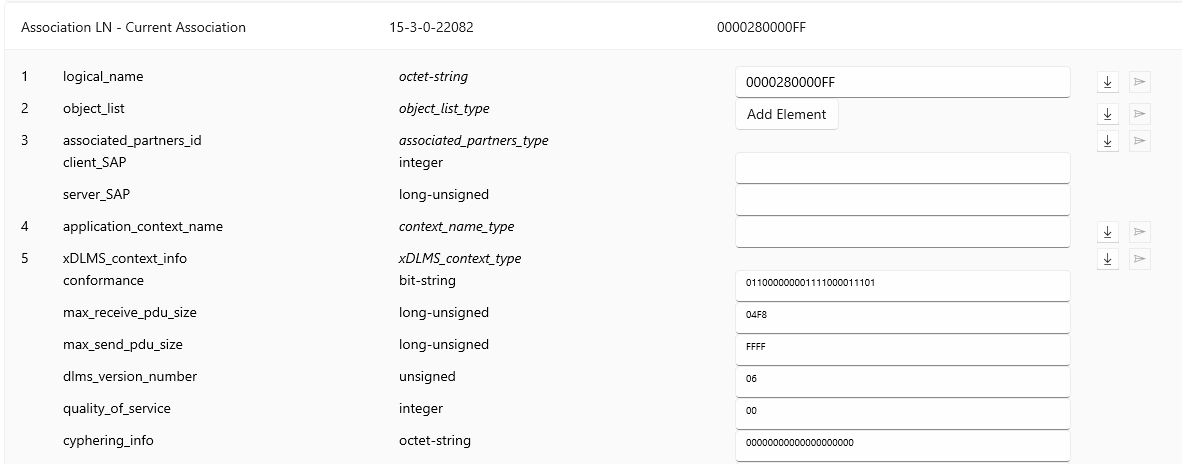
\includegraphics[width=1.0\textwidth]{gfx/AttributeReadExample.png}
   \caption{
      Ausschnitt aus DlmsQuickAccess zum Lesen von Strukturen
      }
      \label{fig:AttributeReadExample}
   \end{figure}
In Abbildung \ref{fig:AttributeReadExample} ist ein Attribut abgebildet, welches ausgelesen wurde.
Dabei ist ersichtlich, dass alle Felder des Struktur \textit{xDLMS\_context\_type} mit Name und Typ beschriftet sind.

Bei der Integration der \textit{InfraLib} in die Solution musste festgestellt werden, dass zwar einige Unit Tests vorhanden sind, jedoch nur geringe Teile des Codes getestet sind.
Da einige Fehler im Parsing-Code gefunden wurde, wurden einige Modul Tests geschrieben, welche das Zusammenspiel der verschiedenen Komponenten von XML-Files bis Adapter testen.

% TODO evtl schrieben, wie und wieso InfraLib eingebunden wurde (NUGET etc)

\subsection{Schreiben von Attributen}
\dq  Die Benutzerschnittstelle soll das Schrieben von Attributwerten sowie ausführen von Methoden unterstützen.\dq

\subsubsection{Ziel}
In der vorherigen Story wurde das Lesen von Attributen über die Benutzerschnittstelle implementiert.
Ziel dieser Story ist es, dass über die selbe Schnittstelle Schreibbefehle ausgeführt werden können.
Ebenfalls soll es möglich sein, dass Methoden ausgeführt werden können.

\subsubsection{Vorgehen und Schwierigkeiten}
Um nebst dem Lesen auch das Schrieben von Attributen über die Benutzerschnittstelle steuern zu können mussten entsprechende \textit{Button} Controls hinzugefügt werden.
Die meisten bestehenden Komponente wurden bereits zuvor so entwickelt, dass das Schreiben ebenfalls unterstützen.
In der Vorgehensbeschriebung zur vorgehenden Story wurde beschrieben, wie das Datenformat der \ac{ATS} in eine Klassenstruktur überführt wurden.
Um Daten zu schrieben, musste dieser Prozess umgekehrt werden.

\begin{figure}
   \centering
   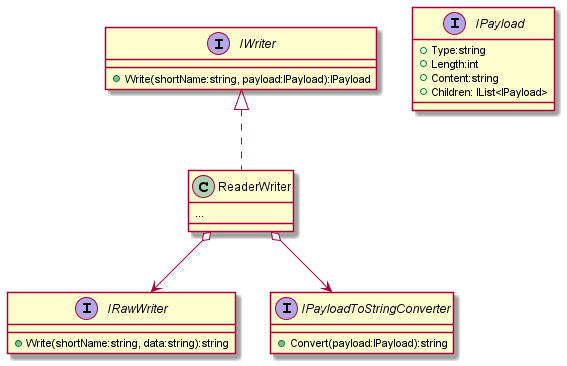
\includegraphics[width=1.0\textwidth]{gfx/payloadTostriing.png}
   \caption{
      Klassendiagramm zur Writer Klasse
      }
      \label{fig:writer}
   \end{figure}
Dies wurde mit der \textit{Writer} Klasse, welche in Abbildung \ref{fig:writer} aufgezeigt ist, implementiert.

Um Methoden auszuführen muss ein Schreibbefehl ausgeführt werden.
Die Parameter der Methode werden als Payload mitgegeben.
So kann die \textit{Writer} Klasse auch für das Ausführen von Methode verwendet werden.
Die Darstellung der Methoden in der Benutzeroberfläche musste um Eingabefelder für die Parameter und ein \textit{Button} Control für das Starten der Ausführung ergänzt werden.
Dabei konnten Element wiederverwendet werden, welche auch bei Attributen eingesetzt werden.
\begin{figure}
   \centering
   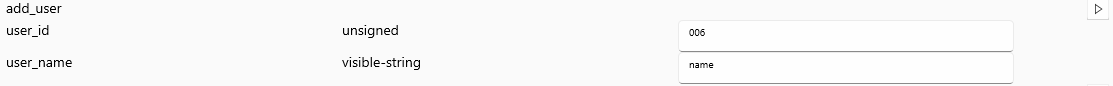
\includegraphics[width=1.0\textwidth]{gfx/addUserMethod.png}
   \caption{
      Ausschnitt aus DlmsQuickAccess der Methode add\_user
      }
      \label{fig:addUserMethod}
   \end{figure}



\subsection{Integration Tests}
Währen dieses Sprints musste oft die ganze Anwendung gestartet werden, um die Integration neuer Funktionen zu testen.
Deshalb wurde für die Validation der Stories dieses Sprints erste Integration Tests geschrieben.
Diese sind so aufgebaut, dass sie bis auf die Benutzerschnittstelle alle Teile der Applikation aufgesetzt werden.
Es wird also das Zusammenspiel der ViewModels mit dem Model getestet.

\subsection{Erster richtiger Release}\label{firstRelease}
Bereist ein Arbeitstag vor Sprintende waren alle geplanten Stories fertiggestellt.
Da die Applikation bereits erste Funktionalität beinhaltet, wurde diese Released den Zukünftigen Benutzern in einer Demo präsentiert.
Die Resonanz dabei war positiv.
Der Release beinhaltete jedoch noch einige Limitierungen.
So wird beispielsweise nur ein spezifisches Version eines Produktes, \textit{Ref\_MMI3}, unterstützt.
Als erste Benutzer den DlmsQuickAccess installierten und starteten stürzte dieser direkt ab.
Im nächsten Sprint sollen diese Abstürze untersucht sowie die Unterstützung von weiteren Produkttypen sichergestellt werden.

\newpage
\section{Sprint 3}
Der Fokus des dritten Sprints liegt bei der Verbesserung der Benutzererfahrung.
Das Ziel ist es, dass die Anwendung danach für die täglichen Arbeiten der Entwickler eingesetzt werden kann.
Dazu sind die folgende beiden Stories geplant:
\begin{itemize}
   \item DlmsQuickAccess soll mehrere, unterschiedliche Stromzählermodelle unterstützen.
   \item Ein Lese- oder Schreibbefehl soll nur dann abgesetzt werden können, wenn dieser laut Object Model vom jeweiligen Objekt unterstützt wird.
\end{itemize}

% Die grösste Lücke besteht aktuell noch darin, dass es nicht möglich ist, zwischen verschiedenen Zähler-Modellen zu wechseln.
% Es ist lediglich möglich mit dem Referenzprodukt "Ref\_MMI3" zu kommunizieren.



\subsection{Unterstützung für unterschiedliche Stromzählermodelle}
\dq  DlmsQuickAccess soll mehrere, unterschiedliche Stromzählermodelle unterstützen.\dq
\subsubsection{Ziel}
Im Abschnitt \ref{picasso} wurde erwähnt, das die Picasso Platform über mehrere Referenzprodukte verfügt.
Drei dieser Referenzprodukte, namentlich \textit{Ref\_IMS1}, \textit{Ref\_NMS2} und \textit{Ref\_MMI3}, werden für die Arbeiten an der Platform täglich verwendet.
Das Ziel dieser Story ist es, dass DlmsQuickAccess mit allen drei kommunizieren kann.
Im Bezug auf die \ac{DLMS} Kommunikation unterscheiden sich diese in zwei Dingen.
Erstens werden verschiedene Kommunikationskanäle verwendet. 
Während bei \textit{Ref\_MMI3} seriell mittels optischem Auslesekopf kommuniziert wird, wird bei \textit{Ref\_NMS2} eine \ac{TLS} Verbindung aufgebaut.
Der zweite Unterschied ist das Objekt Model, welches je nach Produkt andere Objekte enthält.
Damit die Story als erledigt betrachtet werden kann sind noch folgende Punkte zu beachten:
\begin{itemize}
   \item Die Konfiguration eines Produkts soll in einer Datei abgespeichert werden. Wir diese Datei angeklickt, so soll sich der DlmsQuickAccess mit der entsprechend konfiguriert öffnen. % todo evtl file agnostic formulieren
   \item Wird der DlmsQuickAccess ohne Produkt Konfiguration gestartet, so soll eine Auswahl von zuvor geöffneten Konfigurationen angezeigt werden.
   \item Den Benutzern sollen funktionierende Konfigurationen für die drei genannten Referenzprodukte bereitgestellt werden.
   \item Auf der Landis+Gyr internen Wiki soll ein Artikel geschrieben werden, welche Auskunft über DlmsQuickAccess und die Konfigurationsdateien gibt.
\end{itemize}

\subsubsection{Vorgehen und Schwierigkeiten}\label{s3configvorgehen}
Wie in Abschnitt \ref{firstRelease} beschrieben, funktioniert die Anwendungen bisher nur mit dem Produkt \textit{Ref\_MMI3}.
Dies hat damit zu tun, das einige produktspezifische Dateien bisher mit der Anwendung ausgeliefert werden und somit nicht anpassbar sind.
Eine dieser Dateien ist das Object Model als XML. 
Dieses wird, wie im Abschnitt \ref{visualizeOM} erläutert, für die Visualisierung der einzelnen Objekte benötigt und unterscheidet sich von Produkt zu Produkt.
Der Kommunikationscode des \ac{ATS} benötigt ein File mit der Konfiguration des Kommunikationskanals, dieses wird \textit{SetupHW} genannt.
Das \textit{SetupHW} File referenziert eine Adressliste, welche relativ zu ihm abgelegt sein muss.
Da alle Produkte der Picasso Platform mit dem \ac{ATS} getestet werden sind alle benötigten Konfigurationsdateien bereits vorhanden.
Für die Referenzprodukte sind sie im Repository der Testscripts abgelegt.

Der bisherige Ansatz, die Dateien als Teil der Anwendung an die Benutzer auszulieferen, hat nur einen Vorteil.
Die Anwendung kann nach der Installation direkt verwendet werden. Es werden keine weiteren Dateien oder manuelle Konfigurationen benötigt.
Der Nachteil, dass bei jeder Änderung an der Konfiguration eine neue Version der Applikation erstellt und veröffentlicht werden muss überwiegt diesen jedoch, da beispielsweise das Object Model regelmässig verändert wird.
Weitere Nachteile wären, dass um mit einer älteren Version der Firmware Kommuniziert werden kann jeweils eine ältere Version des DlmsQuickAccess installiert werden müsste.

Der zu ersetzende \ac{DMT2} wird über Textfiles konfiguriert.
Um das Produkt zu wechseln, muss jeweils das entsprechende Textfile importiert werden.
Diese Textfiles sind im Repository der Firmware abgelegt somit versioniert.
Die importierte Konfiguration bleibt jeweils sitzungsübergreifend erhalten.
Dies wurde von den Nutzer als unpraktisch gemeldet, da beim Start der Anwendung nicht ersichtlich ist, welche Konfiguration aktiv ist.

Da auch andere Konfigurationen, wie beispielsweise jene des Debuggers oder des FlashTools im Repository des Firmwarecodes abgelegt sind, soll auch jene des DlmsQuickAccess dort verwaltet werden.
Die benötigten Object Models sind ebenfalls bereits Teil des Repository.
Im Picasso Projekt ist \ac{YAML} die bevorzugte Sprache für Konfigurationsdateien.

Basierend auf diesen Überlegungen und Hintergründen wurde folgende Lösung entwickelt:

Für jedes Produkt wird eine Konfigurationsdatei erstellt.
Der Name dieser endet auf .dlmsquickaccess.
Ihre Struktur sieht wie folgt aus:
\begin{verbatim}
Name: Ref_NMS2
ObjectModel: ObjectModel\\ObjectModel_Ref_NMS2.xml
SetupHW: SetupHW1Ref_NMS2.xml
\end{verbatim}
Die Konfigurationsdateien der Referenzprodukte werden im Repository der Firmware abgelegt.
Das \textit{SetupHW} File wird vom Repository der Testscripts in jedes der Firmware kopiert.
Die Applikation wird so angepasst, dass sie mittels Klick auf eine Konfigurationsdatei gestartet werden kann.
Dabei wird jeweils direkt die entsprechende Konfiguration angewendet.

Diese Lösung ermöglicht eine flexible Konfiguration der Produkte.
Dass das \textit{SetupHW} File aus dem Testscript Repository kopiert und somit manuell gepflegt werden muss ist nicht optimal, bietet jedoch den Vorteil, dass keine direkte Abhängigkeit zu weiteren Repositories besteht.

Wie beschrieben wurde die Anwendung so angepasst, dass sie direkt über eine .dlmsquickaccess Datei gestartet werden kann.
Für den Fall, dass sie ohne eine solche gestartet wird, wurde ein neues Fenster implementiert.
Dieses listet alle bisher geöffneten Konfigurationen auf, welche direkt gestartet werden können.
Des weiteren war es geplant, dass mittels Filepicker eine Konfiguration gesucht und geöffnet werden kann.
Dies konnte so jedoch nicht umgesetzt werden.
Die dazu benötigte Komponente von WinUI3, \textit{FileOpenPicker}, funktionierte zu jenem Zeitpunkt nur fehlerhaft\footnote{https://github.com/microsoft/WindowsAppSDK/issues/1188}.


Die neuen Konfigurationsfiles ermöglichen das einfache Wechseln zwischen verschiedenen Produkten.
Als versucht wurde mit einem \textit{Ref\_NMS2} Zähler zu kommunizieren, führte dies regelmässig zu Fehler.
Wurden die Integrationstest mit einem \textit{Ref\_NMS2} Gerät ausgeführte, so schlug jeweils jeder zweite Test fehl.
Dies wurde von der \ac{TLS} Kommunikation verursacht, welche nach dem Kommunizieren nicht richtig beendet wurde.
Für die Tests konnte das Schliessen der Verbindung jeweils in einer \textit{TestCleanup} Funktion aufgerufen werden.
In der Applikation konnte der \textit{OnClose} Event der \textit{Window} Klasse abonniert werden um die Verbindung beim Schliessen des Fensters zu beenden.
Dieser Event wird jedoch nur dann ausgelöst, wenn die Applikation vom User geschlossen wird und nicht wenn sie abstürzt.


An Ende des Sprints konnte diese Story  nicht geschlossen werden, da sich die Konfigurationsdateien noch nicht im Repository der Firmware befanden.
Der entsprechende Commit wartete noch auf ein Review.
Da dies direkt zu Beginn des nächsten Sprints erfolgte und alle anderen Arbeiten in diesem Sprint erledigt werden konnten, wird diese Story im Text zum Sprint 4 (\ref{sprint4}) nicht erwähnt.


\subsection{Deaktivieren von Lese- und Schreibknöpfen}
Das Feld \textit{Access Rights} im Object Model gibt an, ob ein Attribut gelesen und/oder geschrieben werden kann.
Für diese Story wurde die Benutzerschnittstelle so angepasst, dass die Lese- und Schreibknöpfe nur bei jenen Attributen aktiv sind, bei denen die entsprechende Operation möglich ist.
In Abbildung \ref{fig:logicalNameAttribute} ist ein \textit{logical\_name} Attribut gezeigt, welches nur gelesen und nicht geschrieben werden kann.

\begin{figure}[H]
   \centering
   
\includegraphics[width=1.0\textwidth]{gfx/logicalNameAttribute.png}
   \caption{
      Ausschnitt aus DlmsQuickAccess welcher ein einzelnes Attribut zeigt, welches gelesen, jedoch nicht geschrieben werden kann.
      }
      \label{fig:logicalNameAttribute}
   \end{figure}
\newpage
\section{Sprint 4}\label{sprint4}
Nach dem dritten von sechs Sprints sind die Grundfunktionen des DlmsQuickAccess implementiert.
In diesem Sprint begann die zweite Hälfte des Projekts und die Arbeit am ersten Zusatzfeature.


\subsection{Favoriten}

\subsubsection{Ziel}
In der Vorbereitungsphase wurde eine Umfrage bei den zukünftigen Nutzern des DlmsQuickAccess durchgeführt.
Wie in Abschnitt \ref{survey} erklärt priorisierten sie dabei mögliche Zusatzfeatures.
Die Funktion, bestimmte Objekte, Attribute oder Methoden als Favoriten markieren und so vereinfacht abrufen zu können erhielt von den Nutzern die höchste Priorität.
Zun den Akzeptanzkriterien der Story gehören folgende Punkte:
\begin{itemize}
   \item Der Benutzer kann Objekte, Attribute und Methoden zu den Favoritenlisten hinzufügen und wider entfernen.
   \item Favorisierte Attribute und Methoden sollen in einer gemeinsam Liste, Objekte in einer eigenen, dargestellt werden.
   \item Neue Einträge sollen jeweils am Ende der Liste erscheinen.
   \item Favorisierte Attribute und Methoden des selben Objekts sollen gruppiert dargestellt werden. Ihre Reihenfolge soll jener innerhalb des Objekts entsprechen.
   \item Die Favoriten sollen Sitzungs- und Produktübergreifend gespeichert werden.
\end{itemize}


\subsubsection{Vorgehen und Schwierigkeiten}
Damit die Favoriten  Sitzungs- und Produktübergreifend bestehen bleiben, muss eine eindeutige Identifikation der favorisierten Objekte persistiert werden.
Als Identifikation bietet sich der Obis Code des Objektes an.
Dieser ist standartisiert und ändert sich von Produkt zu Produkt nicht.
Bei Attributen und Methoden kann der Obis Code in Kombination mit dem Index des Attributes rsp. der Methode für die Identifikation verwendet werden.
Die Obis Codes und Indizes werden dann im \textit{AppicationDataContainer}\footnote{https://docs.microsoft.com/en-us/uwp/api/windows.storage.applicationdatacontainer} gespeichert.
Dabei handelt es sich um einen Key-Value-Store.
Da dieser vom Betriebssystem verwaltet wird, müssen sich bei der Entwicklung keinerlei Gedanken über Dinge wie Files oder Schreibzugriff gemacht werden müsse.

Damit der Benutzer Steuern kann, welche Element zu seinen Favoriten gehören, wurden Objekte, Attribute und Methoden in der Benutzerschnittstelle um das \textit{CanBeFavoriteControl} erweitert.
Dieses besteht aus einem Knopf, mit welchem ein Element favorisiert oder entfavorisiert werden kann.
Das Icon des Knopfs gibt Auskunft darüber, ob das Element bereits Favorit ist oder nicht.
In Abbildung \ref{fig:objectModelWithFavorites} ist das \textit{CanBeFavoriteControl} auf der rechten Seite der Objekte zu sehen.
Das erste Objekt ist nicht favorisiert, das zweite schon.

\begin{figure}
   \centering
   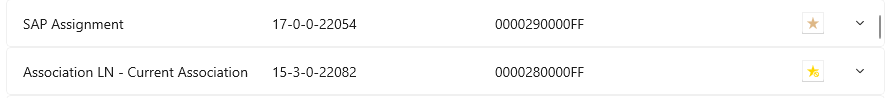
\includegraphics[width=1.0\textwidth]{gfx/objectModelWithFavorites.png}
   \caption{
      Ausschnitt aus DlmsQuickAccess: Ein Objekt ist favorisiert, das andere nicht.
      }
   \label{fig:objectModelWithFavorites}
\end{figure}

Ein Konzept, um die favorisierten Elemente darzustellen ist im Abschnitt \ref{uifavorites} beschrieben.
Dieses wurde im Rahmen dieser Story umgesetzt.
Ursprünglich war geplant, dass lediglich die Namen der favorisierten Objekte aufgelistet werden sollen.
Werden diese angeklickt, so soll das entsprechende Objekt im bereits bestehenden Object Model angezeigt und fokussiert werden.
Dies liess sich so jedoch technisch nicht umsetzten.
Um in der Liste ein bestimmtes Element fokussieren zu können, wir eine Referenz auf dieses benötigt.
Die Instanzen der Controls werden jedoch nicht im C\# Code der Anwendung erstellt, sonder deklarativ mittels XAML.
Deshalb war es nicht möglich, an eine Referenz des gewünschten Controls zu gelangen.

So musste die Idee mit dem Fokussieren verworfen werden.
Stattdessen werden die ganzen Objekte, inklusive Attribute und Methoden, in der Liste der Favoriten dargestellt.
In Abbildung \ref{fig:favoritesUi} ist Liste der favorisierten Objekte gezeigt.
Für die Objekte werden die gleichen Controls wie im Object Model verwendet.
So können die Objekte ebenfalls ein- und ausgeklappt werden.
In der Abbildung ist dies am Beispiel des Objekts \textit{Password Supervision} zu sehen.

\begin{figure}
   \centering
   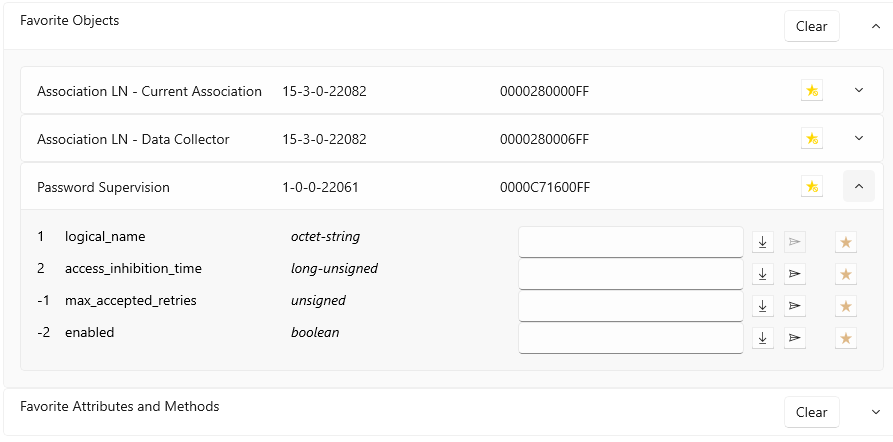
\includegraphics[width=1.0\textwidth]{gfx/favoritesUi.png}
   \caption{
      Die Liste der favorisierten Objekte mit bestehend aus einem Objekt
      }
   \label{fig:favoritesUi}
\end{figure}

Werden einzelne Attribute oder Methoden favorisiert, so erscheinen sie in der Komponente \textit{Favorite Attributes and Methods}, welche in Abbildung \ref{fig:favoriteAttribtuesAndMethods} gezeigt wird.
Die Attribute und Methoden werden jeweils unterhalb des Names des Objektes zu dem sie gehören, angezeigt.
Dies ermöglicht es, dass mit ausgewählten Attribute oder Methoden unterschiedlichster Objekte gearbeitet werden kann, ohne dass hin und her gescrollt werden muss.
\begin{figure}
   \centering
   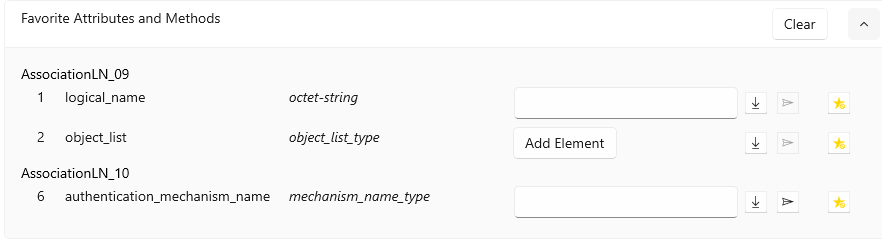
\includegraphics[width=1.0\textwidth]{gfx/favoriteAttributeAndMethods.png}
   \caption{
     Auflistung der favorisierten Attribute und Methoden
      }
   \label{fig:favoriteAttribtuesAndMethods}
\end{figure}

Die Views des Object Model und jener der Favoritenliste nutzen die selben ViewModel Instanzen.
Wird bei einem Element aus der Favoritenliste ein Lesebefehl ausgeführt, so wird der gelesene Wert auch im Object Model angezeigt.
\newpage
\section{Sprint 5}
Im fünften Sprint wurde zwei weiter Zusatzfeatures eingeplant, welche von den Nutzern gewünscht wurden.
Eine weitere Story befasst sich mit einer kleinen Verbesserung des Object Models.
Dies sind die Stories:
\begin{itemize}
   \item Implementation einer Suchfunktion für das Object Model
   \item Implementation einer Filterfunktion für das Object Model
   \item Das Lesen und Schrieben von Enum Werten soll verbessert werden.
\end{itemize}

\subsection{Suchfunktion}
\dq Implementation einer Suchfunktion für das Object Model\dq
\subsubsection{Ziel}
Die Object Models bestehe aus mehreren hundert Objekten und tausenden Attributen und Methoden.
Eine Suchfunktion soll das Finden eines spezifischen Objekts oder einer Gruppe von Objekten erleichtern.
Ebenfalls soll es mögliche sein, bestimmte Attribute oder Methoden zu finden, ohne die dazugehörige Klasse zu kennen.
Bei der Suche soll nach Name, Titel und Obis Code der Objekte gesucht werden.
Für Attribute und Methoden soll jeweils nur der Name verwendet werden.
Die Gross- und Kleinschreibung soll dabei ignoriert werden.
Dass ein Element in den Suchergebnissen erscheint muss der Suchbegriff vollständig enthalten sein.

\subsubsection{Vorgehen und Schwierigkeiten}
Im Abschnitt \ref{searchandfilterUiSktech} wird ein Konzept für die Darstellung der Such- und Filterkomponente erklärt.
Für diese Story wurde die Benutzerschnittstelle für die Suche nach diesem Konzept umgesetzt.
Der geplante Platz für die Filterkomponente wurde frei gelassen, da diese in der Folgestory implementiert wird.
In Klassendiagramm \ref{fig:objectModelVMClassDiagram} ist das Interface \textit{IObjectModelViewModel} abgebildet.
\begin{figure}
   \centering
   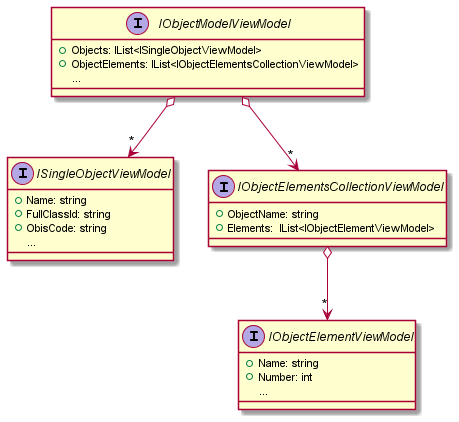
\includegraphics[width=0.7\textwidth]{gfx/OMVM.png}
   \caption{
      Reduziertes Klassendiagramm zu IObjectModelViewModel
      }
      \label{fig:objectModelVMClassDiagram}
\end{figure}
Über diese werden alle Daten abgerufen, welche für die Darstellung der Object Model Komponente benötigt werden.
Die Liste \textit{Objects} beinhaltete alle Objekte, welche im Object Model angezeigt werden.
Die Suchfunktion wie folgt implementieren:
\begin{enumerate}
   \item Die Suche wird mit einem Klick auf den \textit{Find} Knopf gestartet.
   \item Alle \textit{ISingleObjectViewModel} Objekte werden aus der \textit{Objects} Liste entfernt.
   \item Die \ac{COSEM} Objekte werden anhand des Suchtexts gefiltert.
   \item Für jedes verbleibende Objekt wird eine neues \textit{ISingleObjectViewModel} erstellt und der \textit{Objects} Liste hinzugefügt.
\end{enumerate} 
Diese Implementation war funktional ausreichend, jedoch teilweise sehr langsam.
Je mehr Objekte als Suchresultat dargestellt werden mussten, desto langsamer wurde die Suche.
Dies hatte damit zu tun, dass für jedes Objekt ein neues \textit{ISingleObjectViewModel} Objekt erstellt wurde.
Um dies zu verbessern wurde ein Cache eingesetzt, welcher anstelle eines neuen Objekt jeweils ein bestehendes liefert.

Um nicht nach Objekten sondern nach Attributen und Methoden zu suchen, wurde etwas ähnliches implementiert.
Im Klassendiagramm ist das Interface \textit{IObjectElementsCollectionViewModel} aufgezeigt.
Dieses fasst alle Attribute und Methoden einer Klasse zusammen, welche dargestellt werden sollen.
Im Property \textit{ObjectElements} wird eine Liste dieser Objekte gehalten.
Diese wird mit dem gleichen Vorgehen wie bei den Objekten auf jenen Elemente reduziert, welche den Suchkriterien entsprechen.
In Abbildung \ref{fig:searchforClock} ist die Suche nach Attributen und Methoden dargestellt.


\begin{figure}
   \centering
   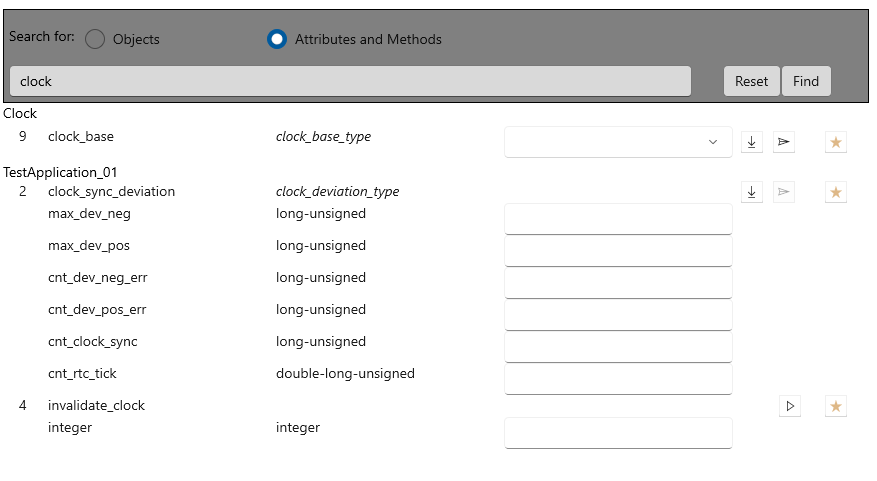
\includegraphics[width=1.0\textwidth]{gfx/searchforclick.png}
   \caption{
      Resultate der Suche nach Attributen und Methoden mit dem Text \dq clock\dq
      }
      \label{fig:searchforClock}
\end{figure}




\subsection{Filterfunktion}
\dq Implementation einer Filterfunktion für das Object Model\dq
\subsubsection{Ziel}
Um Objekte einer bestimmten \ac{COSEM} Klasse anzuzeigen, soll eine Filterfunktion implementiert werden.
Es soll möglich sein, dass nach Class Id, Class Version, Own Class Version und Sub Type gefiltert werden können.
\subsubsection{Vorgehen und Schwierigkeiten}
\begin{figure}
   \centering
   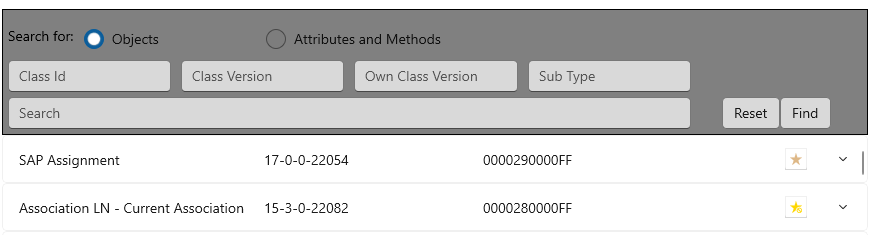
\includegraphics[width=1.0\textwidth]{gfx/searchfilter.png}
   \caption{
      Such- und Filterfunktion aus DlmsQuickAccess 
      }
      \label{fig:searchfilterUIRel}
\end{figure}
Die Filterfunktion wurde bereits bei den Arbeiten an der Suchfunktion berücksichtigt.
In der Benutzerschnittstelle mussten nur noch die zusätzlichen Textfelder hinzugefügt werden.
Abbildung \ref{fig:searchfilterUIRel} zeigt diese.
Der Algorithmus, welcher die \ac{COSEM} Objekte bisher nach Suchtext filtert wurde so erweitert, dass die neu hinzugefügten Parameter berücksichtigt werden.
Dies konnte ohne Schwierigkeiten umgesetzt werden.



\subsection{Enums}
\dq Das Lesen und Schrieben von Enum Werten soll verbessert werden.\dq
\subsubsection{Ziel}
Im \ac{DMT2} sowie in den bisherigen Versionen des DlmsQuickAccess wurden Enums gleich wie andere Zahlenwerte behandelt.
Nutzer der Anwendungen mussten jeweils die Class Description der entsprechenden Klasse abrufen, um die Bedeutung eines bestimmten Werts zu erfahren.
Dies soll verbessert werden, indem anstelle der Nummer die dazugehörige Bezeichnung angezeigt wird.

\subsubsection{Vorgehen und Schwierigkeiten}
Im Text zur Realisierung des zweiten Sprints (\ref{readAttributVorgehen}) wurde erklärt, dass für die optimale Darstellung des Object Models Informationen aus der XML Datei es Object Models um jene der Class Descriptions erweitert wurden.
Zu diesen Informationen gehören auch die Bezeichnungen der Enums.
In Abbildung \ref{fig:enumTypedefword} ist ein Ausschnitt aus einer Class Description gezeigt, welcher die Definition eines Enum-Types beinhaltet.
\begin{figure}
   \centering
   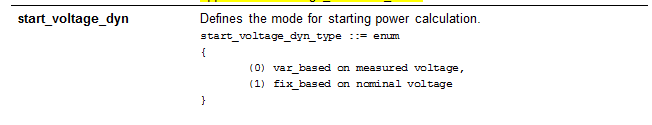
\includegraphics[width=1.0\textwidth]{gfx/enum_typedef_word.png}
   \caption{
      Ausschnitt aus dem Word Dokument einer Class Description
      }
      \label{fig:enumTypedefword}
\end{figure}
In der XML Repräsentation dieser Class Description, welche vom DlmsQuickAccess eingelesen wird, sieht diese Typendefinition wie folgt aus:
\begin{verbatim}
<cm:typedefinition name="start_voltage_dyn_type" base="enum">
   <cm:item name="var_based on measured voltage" value="0" />
   <cm:item name="fix_based on nominal voltage" value="1" />
</cm:typedefinition>
\end{verbatim}

Im Abschnitt \ref{readAttributVorgehen} wurde erklärt, dass das Adapter Pattern verwendet wurde, um die Class Descriptions in die gewünschte Klassenstruktur zu überführen.
Als versucht wurde, auf die einzelnen Enum Werte zuzugreifen, traten Fehler bei der Implementation der Adapter auf.
Diese zeigten sich dann, wenn mehrere Typendefinitionen ineinander verschachtelt sind.
Das kommt beispielsweise dan vor, wenn es sich beim Typen eines Attributes um ein Array handelt, wessen Elemente jeweils Strukturen sind, welche ein Feld von Type Enum enthalten.

Um das Problem zu lösen, wurde es versucht mittels Unit Tests zu reproduzieren.
Dies war sehr umständlich, was auf eine tiefe Testbarkeit dieser Adapterklassen hinwies.
In Abschnitt \ref{testability} wurde erklärt, dass schwer testbarer Code auf tiefe Qualität hindeutet.
Deshalb wurden einige dieser Adapter Klassen durch neue, bessere Implementationen ersetzt.

Rückblickend muss gesagt werden, dass das Verwenden des Codes der \textit{InfraLib} nicht zu den erhofften Zeitersparnissen geführt hat.
Die Library war nicht ausreichend getestet und einige erwarteten Funktionen fehlten ganz.
Eine von Grund auf eigene Implementation für das Parsing der Class Description wäre vermutlich mit weniger Zeitaufwand verbunden gewesen und hätte zu einer besseren Lösung geführt.

\newpage
https://www.c-sharpcorner.com/UploadFile/78607b/difference-between-ienumerable-icollection-and-ilist-interf/

https://books.google.ch/books?hl=de&lr=&id=pKVFDwAAQBAJ&oi=fnd&pg=PA3&dq=software+quality+assurance&ots=Gd9uAgA9c3&sig=7e-9sSZofRdKz3-WDZYGtqzuigE&redir_esc=y#v=onepage&q=software%20quality%20assurance&f=false
\newpage